\chapter{Abstrahieren} 

Bei der Analyse und Beobachtung artikulatorischer, akustischer und perzeptiver Aspekte gesprochener Sprache fällt die große Variabilität auf. Sprecher unterscheiden sich in ihrer Produktion (und folglich Akustik) von Sprachlauten und auch innerhalb eines Sprechers gibt es jede Menge Unterschiede: Kein Laut  wird jemals identisch produziert. Um die Funktion von Sprachlauten innerhalb einer Sprache und deren Lautinventar zu ermitteln, ist es nötig, die Variation auszuklammern und zu abstrahieren.

\section{Stichworte zur Vorlesung \em{Einführung in die Phonologie}}

Kontrast, Phon, Phonem, Allophon, freie Variante, komplementäre Distribution\dots $\rightarrow$ {\tt L8\underline{\ }Phonologie.pdf}

\begin{figure}[htbp]
\begin{center}
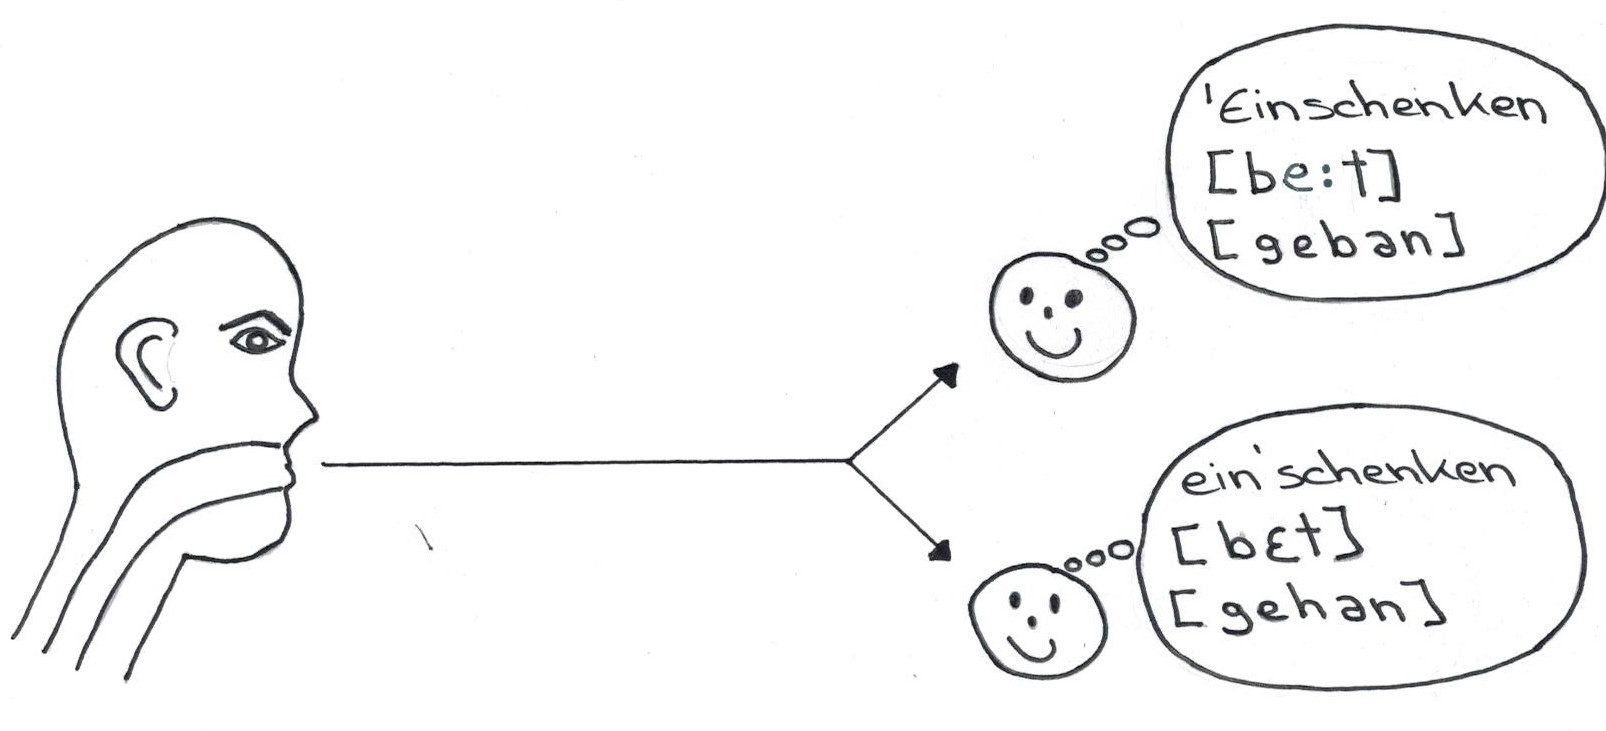
\includegraphics[width=0.6\textwidth]{grafiken/abstrahieren/distinktive-merkmale.jpg}
\label{t6}
\end{center}
\end{figure}




\newpage
\section{Übungen}

1.	Lesen Sie den ausgeteilten Text von Trubetzkoy und stellen sie die ihrer Meinung nach wichtigsten Informationen schematisch dar.\vspace{\fill}


2.	Tragen Sie die Sprachlaute des Deutschen in folgende Tabelle ein und unterstreichen Sie alle Laute, die ihrer Meinung nach Phoneme des Deutschen sind.

\begin{sidewaystable}\centering
\small
\begin{tabular}{|l|l|l|lcr|l|l|l|l|l|l|}  \hline
 & Bilabial & Labiodental & Dental & Alveolar & Postalveolar & Retroflex & Palatal & Velar & Uvular & Pharyngeal & Glottal\\ \hline
Plosive	&	&	&	&	&	&	&	&	&	&	& \\ \hline
Nasal	&	&	&	&	&	&	&	&	&	&	& \\ \hline
Tap or Flap	&	&	&	&	&	&	&	&	&	&	& \\ \hline
Fricative	&	&	&	&	&	&	&	&	& 	&	& \\ \hline
Lateral fricative	&	&	&	&	&	&	&	&	&	&	& \\ \hline
Approximant	&	&	&	&	&	&	&	&	&	&	& \\ \hline
Lateral approximant	&	&	&	&	&	&	&	&	&	&	& \\ \hline


\end{tabular}
\end{sidewaystable}

\newpage
3.	Lesen Sie den ausgeteilten Text von Kohler. Ist der Glottalverschluss Ihrer Meinung nach ein Phonem des Deutschen? Notieren Sie Pro- und Contra-Argumente. \vspace{5cm}\\
